\section{Question 1-3: Dataset and Numner of Cluster} \label{Sec: Question 1}

\subsection{The curse of dimensionality}
The curse of dimensionality dictatates that, as the number of dimensions grows, the difference between the minimum distance and the maximum distance approaches 0, the pattern in the dataset hence does not make sense anymore \cite{koppen2000curse}.
To illustrate the phenomena, we pick a random datapoint $P$ within the dataset $Q$.
We start with 2 features and increase to 10, for each loop, we compute the distance from $P$ to each point in $Q$.

\begin{lstlisting}[language=Python]
random_index = int(np.floor(np.random.random()*len(data)))
P = data.iloc[random_index].to_numpy()
Q = data.drop(axis=0, index=random_index).to_numpy()

deltas = []

for N in range(2, 11):

    p = P[:N]
    q = Q[:,:N]


    diffs = [np.linalg.norm(q-p) for q in q]
    mxd = max(diffs)
    mnd = min(diffs)
    delta = math.log10(mxd-mnd)/mnd
    deltas.append( delta )
\end{lstlisting}

As the number of dimensions increases, the difference between maximum distance and minimum distance became smaller and smaller exponentially as illustrated in Figure \ref{Fig: curse of dim}.
Thus the given dataset suffers from the curse of dimensionality.

\begin{figure}
    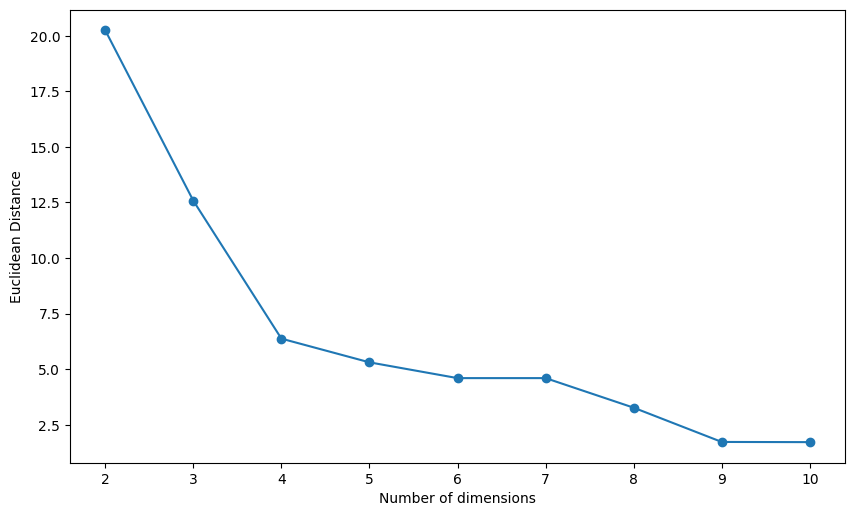
\includegraphics[width=\textwidth]{Appendices/curse-dim.png}
    \caption{The Euclidean distance of a random value to the rest of the dataset for each feature.}
    \label{Fig: curse of dim}
\end{figure}

\subsection{Grouping Travellers and Cluster Evaluation Techniques}
To find the group of travellers from the given dataset, we can categorize users into groups based on different factors.
In this case, we can group users based on their rating in different categories.

The KMeans clustering algorithm to identify such groups of travellers.
For example, the scripts belows will partition the data into two groups.

\begin{lstlisting}[language=Python]
kmeans_example = KMeans(n_clusters=2).fit(data.to_numpy())

print(f'There are two clusters, their centroids are: \n{kmeans_example.cluster_centers_[0]} \nand \n{kmeans_example.cluster_centers_[1]}')

>>> There are two clusters, their centroids are: 
[0.90599476, 1.41947644, 1.82939791, 0.58280105, 1.18, 2.18356021, 3.1871466,  2.80489529, 1.52609948, 2.60157068] 
and 
[0.88501672, 1.30989967, 0.49198997, 0.50036789, 0.78625418, 1.62528428, 3.17697324, 2.8543311, 1.59712375, 2.92548495]
\end{lstlisting}

So far, we know that users can be classified into two groups using KMeans algorithm.
However, there must be a number of cluster that is optimal for the dataset.
We can to find the optimal number of traveller groups, by using various of cluster validation techniques.
\emph{The elbow method} \cite{syakur2018integration} is a widely used for calculate the optimal number of clusters.
For different values of $k$, we calculate the Within-Cluster-Sum of Squared (wss) Errors and chose the first $k$ values for which the error values start to diminish.

We obtain the folloing graph (see Figure \ref{Fig: WSS}) for WSS values of our dataset for different $k$ number of clusters.
The plot took shape of an arm, and we can chose the optimal at the elbow.
It is suggested that the optimal values $k$ can be chosen within the range $[7, 10]$, as highlighted in the plot.

\begin{figure}
    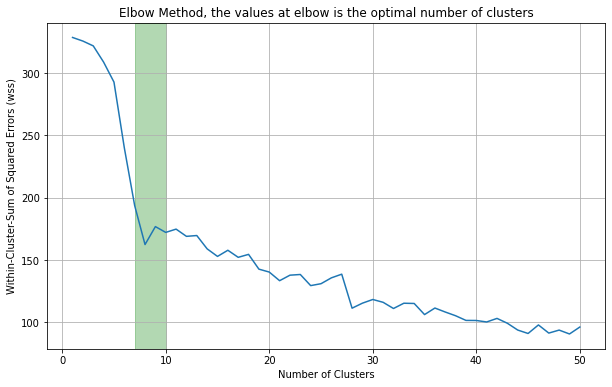
\includegraphics[width=\textwidth]{Appendices/elbow.png}
    \caption{WSS values of the given dataset for different $k$ number of clusters.}
    \label{Fig: WSS}
\end{figure}

\subsection{Silhouette Method with KMeans Algorithm}
Compare to the elbow method, the \emph{silhouette score} measures the similarity of a point to it own cluster compared to the other clusters \cite{shahapure2020cluster}.
The silhouette score is calculated with the function \lstinline{silhouette_score()} from sklearn library.
We aim to choose $k$ values for the highest silhouette scores.

We obtain the silhouette scores of KMeans clustering algorithm for our dataset with different $k$ number of clusters as Figure \ref{Fig: Sil Kmeans}.
The result shows that $k=2$ clusteres would maximize the average silhouette score for the dataset (highlighted as red dot).
Otherwise, we can chose the second peak, at $k = 8$ (highlighted as orange dot).

\begin{figure}
    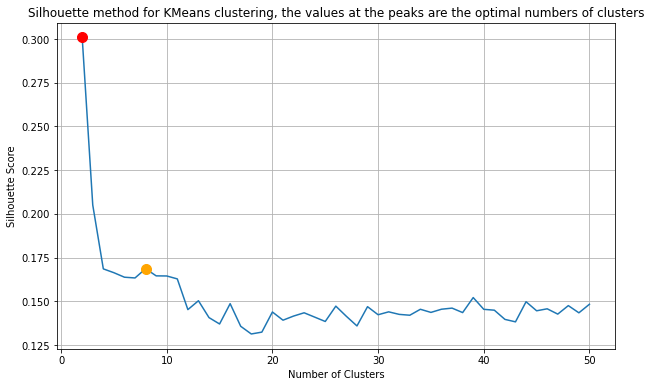
\includegraphics[width=\textwidth]{Appendices/Sil-Kmean.png}
    \caption{Silhouette score for clusters using KMeans algorithm}
    \label{Fig: Sil Kmeans}
\end{figure}

\subsection{Silhouette method with Spectral Clustering}
Spectral Clustering is another clustering algorithm.
Compare to KMeans algorithm wich groups the data based on how close they are toward the cluster center (compactness approach), Spectral clustering algorithm use the connectivity approach, wich group the datapoint based on their $\epsilon$ distance to each other \cite{liu2018spectral}.

Applies the Spectral Clustering to calculate Silhouette score gives the results as Figure \ref{Fig: Sil Spec}.
The result shows that $k=2$ clusteres would maximize the average silhouette score for the dataset (highlighted as red dot).
Otherwise, we can chose the second peak, at $k = 5$ (highlighted as orange dot).

\begin{figure}
    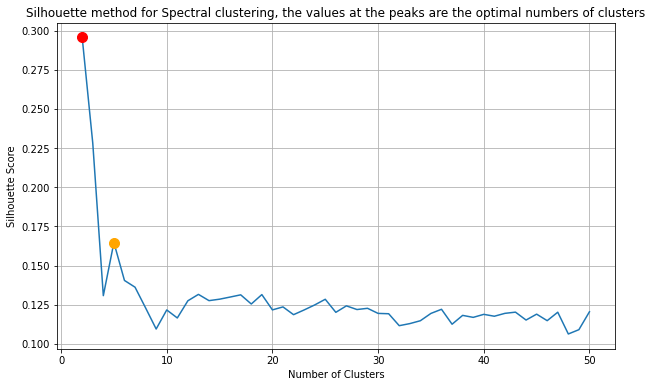
\includegraphics[width=\textwidth]{Appendices/Sil-Spec.png}
    \caption{Silhouette score for clusters using Spectral Clustering algorithm}
    \label{Fig: Sil Spec}
\end{figure}

\subsection{The Optimal Number of Cluster}
We have obtained results as the optimal number of clusters for the dataset based on different clustering algorithms and cluster evaluation techniques.
The findings are summarised as the Table \ref{Tab: cluster and eva result}.
\begin{table}
    \centering
    \begin{tabular}{||c c c c||}
        \hline
        Index & Clustering Algorithm & Evaluation Technique & Optimal $k$ \\
        \hline \hline
        1     & KMeans clustering    & Elbow WSSE           & [7, 10]     \\
        2     & KMeans clustering    & Silhouette Score     & 2, 8        \\
        3     & Spectral clustering  & Silhouette Score     & 2, 5        \\
        \hline
    \end{tabular}
    \caption{Summarised result of Clustering algorithm and evalutaion techniques}
    \label{Tab: cluster and eva result}
\end{table}

The first method (elbow) has zoned the optimal values within the range from 7 to 10 clusters.
However, in the second and third method, we can see that the optimal values are 2, 5, and 8.
The value $k=8$ is within the optimal range [7, 10] from the first method and thus having a reasonable Within-Cluster-Sum of Squared Errors value (marked as blue dot).
Onthe other hand, the values $k=2$ and $k=5$ will result in higher error values (marked as red dot).
In conclusion, the optimal number of cluster is $k=8$ (see Figure \ref{Fig: Optimal})

\begin{figure}
    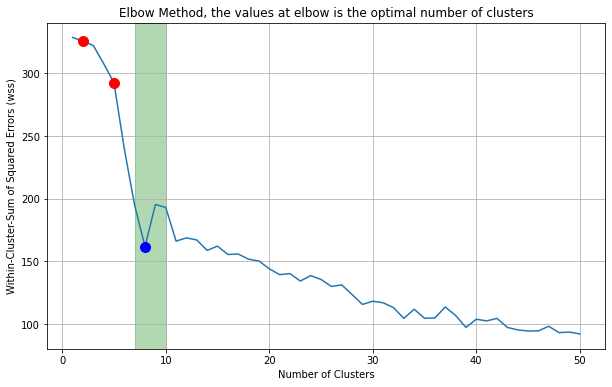
\includegraphics[width=\textwidth]{Appendices/optimalCluster.png}
    \caption{Optimal number of Cluster}
    \label{Fig: Optimal}
\end{figure}
